\documentclass[a4paper, 10pt, ]{article}

\usepackage[slovak]{babel}

% ------------------------------

\usepackage[utf8]{inputenc}
\usepackage[T1]{fontenc}

\usepackage[left=4cm,
            right=4cm,
            top=2.1cm,
            bottom=2.6cm,
            footskip=7.5mm,
            twoside,
            marginparwidth=3.0cm,
            %showframe,
            ]{geometry}

\usepackage{graphicx}
\usepackage[dvipsnames]{xcolor}
% https://en.wikibooks.org/wiki/LaTeX/Colors

% ------------------------------

\usepackage{lmodern}

\usepackage[tt={oldstyle=false,proportional=true,monowidth}]{cfr-lm}
% https://mirror.szerverem.hu/ctan/fonts/cfr-lm/doc/cfr-lm.pdf

% ------------------------------

\usepackage{amsmath}
\usepackage{amssymb}
\usepackage{amsthm}

\usepackage{booktabs}
\usepackage{multirow}
\usepackage{array}
\usepackage{dcolumn}

\usepackage{natbib}

% ------------------------------

\hyphenpenalty=6000
\tolerance=1000

\def\naT{\mathsf{T}}

% ------------------------------

\makeatletter

    \def\@seccntformat#1{\protect\makebox[0pt][r]{\csname the#1\endcsname\hspace{4mm}}}

    \def\cleardoublepage{\clearpage\if@twoside \ifodd\c@page\else
    \hbox{}
    \vspace*{\fill}
    \begin{center}
    \phantom{}
    \end{center}
    \vspace{\fill}
    \thispagestyle{empty}
    \newpage
    \if@twocolumn\hbox{}\newpage\fi\fi\fi}

    \newcommand\figcaption{\def\@captype{figure}\caption}
    \newcommand\tabcaption{\def\@captype{table}\caption}

\makeatother

% ------------------------------

\usepackage{fancyhdr}
\fancypagestyle{plain}{%
\fancyhf{} % clear all header and footer fields
% \fancyfoot[C]{\sffamily {\bfseries \thepage}\ | {\scriptsize\oznacenieCasti}}
\fancyfoot[C]{\sffamily {\bfseries \thepage}{\color{Gray}\scriptsize$\,$z$\,$\pageref{LastPage}}\ | 
\includegraphics[height=5pt]{../../COMMONFILES/KUT_logo_v0.1.pdf}{\scriptsize\KUTporadoveCislo}}
\renewcommand{\headrulewidth}{0pt}
\renewcommand{\footrulewidth}{0pt}}
\pagestyle{plain}

% ------------------------------

\usepackage{titlesec}
\titleformat{\paragraph}[hang]{\sffamily  \bfseries}{}{0pt}{}
\titlespacing*{\paragraph}{0mm}{3mm}{1mm}
\titlespacing*{\subparagraph}{0mm}{3mm}{1mm}

\titleformat*{\section}{\sffamily\Large\bfseries}
\titleformat*{\subsection}{\sffamily\large\bfseries}
\titleformat*{\subsubsection}{\sffamily\normalsize\bfseries}


% ------------------------------

\PassOptionsToPackage{hyphens}{url}
\usepackage[pdfauthor={},
            pdftitle={},
            pdfsubject={},
            pdfkeywords={},
            % hidelinks,
            colorlinks=false,
            breaklinks,
            ]{hyperref}


% ------------------------------

\graphicspath{%
{../fig_standalone/}%
{../../PY/fig/}%
{../../ML/fig/}%
{./fig/}%
}

% ------------------------------

\usepackage{enumitem}

\usepackage{lettrine}

% ------------------------------

\usepackage{lastpage}

\usepackage{microtype}

% ------------------------------

\usepackage{algorithm}
\usepackage[noend]{algpseudocode}
\makeatletter
\renewcommand{\ALG@name}{Algoritmus}
\makeatother
\usepackage{amsmath}
\usepackage{bbold}
\usepackage{calc}
\usepackage{dsfont}
\usepackage{mathtools}
\usepackage{tabto}


\newcommand{\mr}[1]{\mathrm{#1}}
\newcommand{\bs}[1]{\boldsymbol{#1}}
\newcommand{\bm}[1]{\mathbf{#1}}

\newcommand{\diff}[2]{\frac{\Delta #1}{\Delta #2}}
\newcommand{\der}[2]{\frac{d #1}{d #2}}
\newcommand{\parder}[2]{\frac{\partial #1}{\partial #2}}

\newcommand{\argmax}[0]{\mr{argmax}}
\newcommand{\diag}[0]{\mr{diag}}
\newcommand{\rank}[0]{\mr{rank}}
\newcommand{\trace}[0]{\mr{tr}}

\renewcommand{\Re}{\mr{Re}}
\renewcommand{\Im}{\mr{Im}}


\theoremstyle{definition}
\newtheorem{definition}{Definícia}[section]
\newtheorem{theorem}{Veta}[section]
\newtheorem{lemma}[theorem]{Lemma}
\newtheorem{example}{Príklad}[section]
\renewcommand*{\proofname}{Dôkaz}

% ------------------------------


% -----------------------------------------------------------------------------

\def\oznacenieCelku{Kolekcia učebných textov}

% -----------------------------------------------------------------------------


\def\KUTporadoveCislo{dev250624}

\def\oznacenieVerzie{v0.9}
% \def\oznacenieVerzie{\phantom{v1.0}}

\def\mesiacRok{jún 2025}

\def\authorslabel{MT}






% -----------------------------------------------------------------------------

\begin{document}

% -----------------------------------------------------------------------------
% Uvodny nadpis

\noindent
\parbox[t][18mm][c]{0.3\textwidth}{%
\raisebox{-0.9\height}{%
\phantom{.}
\includegraphics[height=18mm]{./COMMONFILES/URKFEIlogo.pdf}%
}%
}%
\parbox[t][18mm][c]{0.7\textwidth}{%
\raggedleft

\sffamily
\fontsize{16pt}{18pt}
\fontseries{sbc}
\selectfont

\noindent
\textcolor[rgb]{0.75, 0.75, 0.75}{\textls[25]{\oznacenieCelku}}
}%

\noindent
\parbox[t][16mm][b]{0.5\textwidth}{%
\raggedright

\color{Gray}
\sffamily

\fontsize{12pt}{12pt}
\selectfont
\mesiacRok

\fontsize{6pt}{10pt}
\selectfont
github.com/OkoliePracovnehoBodu/KUT

\fontsize{8pt}{10pt}
\selectfont
\authorslabel




}%
\parbox[t][16mm][b]{0.5\textwidth}{%
\raggedleft

\sffamily

\fontsize{6pt}{6pt}
\selectfont

\textcolor[rgb]{0.68, 0.68, 0.68}{\oznacenieVerzie}


\fontsize{14pt}{14pt}
\selectfont

\bfseries


\includegraphics[height=12pt]{./COMMONFILES/KUT_logo_v0.1.pdf}%
{%
\textls[-50]{\KUTporadoveCislo}
}%
}%

% -----------------------------------------------------------------------------




\vspace{6mm}

% ---------------------------------------------
\sffamily
\bfseries
\fontsize{18pt}{21pt}
\selectfont

\begin{flushleft}
    Laboratórne zariadenie LMOT:\\ statické vlastnosti
\end{flushleft}

\bigskip

% -----------------------------------------------------------------------------
\normalsize
\normalfont
% -----------------------------------------------------------------------------

\lstset{style=mystyle}










\noindent
\lettrine[lines=1, nindent=1pt, loversize=0.0]{C}{ieľom} 
textu je opis laboratórneho dynamického systému LMOT z hľadiska jeho statických vlastností.


\section{Opis dynamického systému LMOT}

LMOT je laboratórne zariadenie predstavujúce reálny dynamický systém. Pozostáva z malého jednosmerného motora, tachodynama, ktoré je na spoločnom hriadeli s~motorom, a z elektronických obvodov, ktoré zabezpečujú napájanie motora. Elektronickymi obvodmi sú tiež dané dominantné statické a dynamické vlastnosti výsledného systému. Do istej miery je možné tieto vlastnosti meniť manuálnym nastavením príslušného potenciometra.

Systém má jeden vstupný signál a jeden výstupný signál. Výstupný signál je priamo úmerný uhlovej rýchlosti jednosmerného motora, ktorá je snímaná tachodynamom. Vstupný signál ovláda napájanie motora.

Polohou potenciometra je v podstate daná prevádzková podmienka zariadenia. K~dispozícii je signál zodpovedajúci polohe potenciometra a teda tým je k dispozícii informácia o prevádzkovej podmienke systému.

LMOT (čítaj \emph{elmot}) je akronym pre „laboratórny motorček“, prípadne pre „little motor“.



\section{Meranie prevodovej charakteristiky}

V kontexte statických vlastností systému má vo všeobecnosti význam hovoriť o~prevodovej charakteristike systému. Prevodová charakteristika je závislosť ustálených hodnôt výstupného signálu systému od ustálených hodnôt vstupného signálu systému.

Je zrejmé, že prevodová charakteristika sa týka systémov s prívlastkom statické, teda takých, ktoré nie sú astatické.

Prevodová charakteristika, niekde sa nazýva aj statická charakteristika, teda charakterizuje systém len v~ustálených stavoch. Neobsahuje informáciu o dynamike systému.



\subsection{Návrh merania}

Z opisu predmetného dynamického systému vyplýva, že systém má jeden výstupný signál, jeden vstupný signál a manuálne nastaviteľnú prevádzkovú podmienku.

\paragraph{Rozsahy a jednotky signálov}

Vstupný a výstupný signál nadobúdajú hodnoty v~rozsahu $0$ až $10$ pričom ide o~napäťové signály vo voltoch [V].

Prevádzková podmienka systému sa nastavuje manuálne otáčaním potenciometra. Signál o polohe potenciometra nadobúda hodnoty v rozsahu $0$ [V] až $10$ [V].

\paragraph{Voľba ustálených hodnôt vstupov}

O predmetnom systéme je známe, že výstup systému sa ustáli vždy ak sú vstupy systému ustálené. Pre vyšetrovanie ustálených stavov je teda možné využiť celý rozsah vstupného signálu a celý rozsah prevádzkových podmienok.

Návrh uvažuje ustálené hodnoty vstupného signálu uvedené v tabuľke~\ref{tab:ustalene_hodnoty_vstupneho_signalu} a zároveň ustálené hodnoty reprezentujúce prevádzkové podmienky podľa tabuľky \ref{tab:ustalene_hodnoty_podmienok}.


\begin{center}

\vspace{-10pt}    
    
\tabcaption{Ustálené hodnoty vstupného signálu [V]}
\label{tab:ustalene_hodnoty_vstupneho_signalu}

\lstyle

\begin{tabular*}{\textwidth}{@{ \extracolsep{\fill}} ccccccccccc}
\toprule
0 & 1 & 2 & 3 & 4 & 5 & 6 & 7 & 8 & 9 & 10 \\
\bottomrule
\end{tabular*}


\tabcaption{Ustálené hodnoty signálu o prevádkových podmienkach [V]}
\label{tab:ustalene_hodnoty_podmienok}

\lstyle

\begin{tabular*}{\textwidth}{@{ \extracolsep{\fill}} ccccccccccc}
\toprule
0 & 1 & 2 & 3 & 4 & 5 & 6 & 7 & 8 & 9 & 10 \\
\bottomrule
\end{tabular*}

\end{center}


\paragraph{Voľba časového intervalu pre ustálenie výstupu systému}

Empirické skúsenosti so systémom ukazujú, že z praktického hľadiska sa systém ustáli do $15$ sekúnd po zmene na vstupe systému. Ukazuje sa však aj náchylnosť systému k poruchám spôsobeným zväčša mechanickými nedostatkami a vibráciami zrejme spôsobujúcimi zmeny trenia v mechanických častiach systému. Pre pozorovanie a~vyhodnotenie vplyvu týchto porúch v ustálenom stave je časový interval pre ustálenie zvolený na $120$ sekúnd.



\paragraph{Postup merania}

Vzhľadom na uvedené voľby ustálených hodnôt a časového intervalu návrh predpokladá nasledovný postup.

\begin{enumerate}[leftmargin=0pt, labelsep=4mm, itemsep=0pt]
    \item Manuálne nastavenie prevádzkových podmienok na hodnotu z tabuľky~\ref{tab:ustalene_hodnoty_podmienok}.
    \item Postupná zmena vstupného signálu na hodnoty z tabuľky~\ref{tab:ustalene_hodnoty_vstupneho_signalu} so zvoleným časovým intervalom. Takúto postupnú zmenu vyjadruje nasledujúca tabuľka \ref{tab:postupna_zmena_vstupneho_signalu}.
    
\end{enumerate}


\begin{center}

\vspace{-10pt}    

\tabcaption{Postupná zmena vstupného signálu}
\label{tab:postupna_zmena_vstupneho_signalu}

\lstyle

\begin{tabular*}{\textwidth}{@{ \extracolsep{\fill}} cc}
\toprule
Čas zmeny vstupného signálu [s] & Hodnota vstupného signál [V] \\
\midrule
0 & 0 \\
120 & 1 \\
240 & 2 \\
360 & 3 \\
480 & 4 \\
600 & 5 \\
720 & 6 \\
840 & 7 \\
960 & 8 \\
1080 & 9 \\
1200 & 10 \\
\bottomrule
\end{tabular*}

\end{center}

Celková dĺžka merania je teda $1200 + 120 = 1320$ sekúnd a počas tejto doby sú prevádzkové podmienky konštantné.



\section{Získané dáta}

Príklad získaných dát podľa uvedeného postupu je znázornený na nasledujúcom obrázku \ref{fj_01_data_pot0}.  


% \begin{center}
    \begin{figure}[t]

    \vbox{%
        \makebox[\textwidth][c]{%
        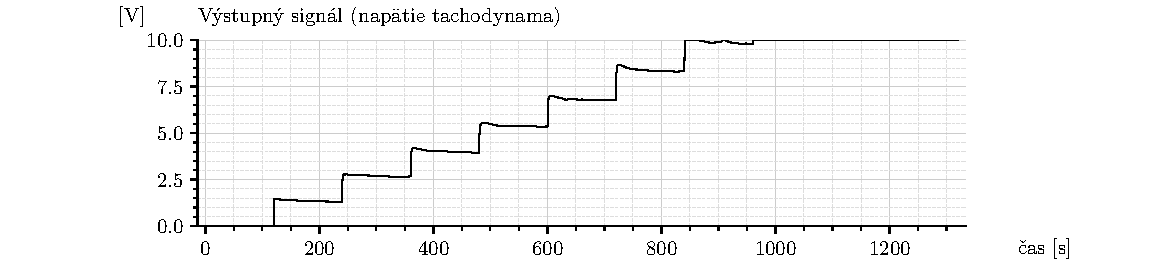
\includegraphics{fj_01_data_pot0_panel_1.pdf}
        }

        \makebox[\textwidth][c]{%
        
\includegraphics{fj_01_data_pot0_panel_3.pdf}
        }

        \makebox[\textwidth][c]{%
        
\includegraphics{fj_01_data_pot0_panel_2.pdf}
        }

        % \figcaption{ 
        \caption{
            Získané dáta pre vstupný signál a výstupný signál systému LMOT pri manuálne nastavenej prevádzkovej podmienke $0$ [V].
        }
        \label{fj_01_data_pot0}
    }%vbox

    \end{figure}
% \end{center}

Získané dáta pre ostatné prevádzkové podmienky sú uvedené v~prílohách tohto textu. Vizualizované sú tu tak dáta pre všetky prevádzkové podmienky, ktoré sú v~tabuľke~\ref{tab:ustalene_hodnoty_podmienok}.












\section{Spracovanie dát pre prevádzkovú podmienku 0 [V]}

\subsection{Vykreslenie ustálených úsekov}

Zo získaných dát na obrázku \ref{fj_01_data_pot0} je potrebné vyňať úseky, počas ktorých sú výstupný a~vstupný signál ustálené. V tomto prípade nech za ustálený stav sa považuje posledných 30 \% zvoleného časového intervalu pre ustálenie, teda posledných 36 sekúnd z celkových 120 sekúnd. Takto vyňaté úseky sú znázornené na obrázku \ref{fj_02_data_pot0}.

% \begin{center}
    \begin{figure}[t]

    \vbox{%
        \makebox[\textwidth][c]{%
        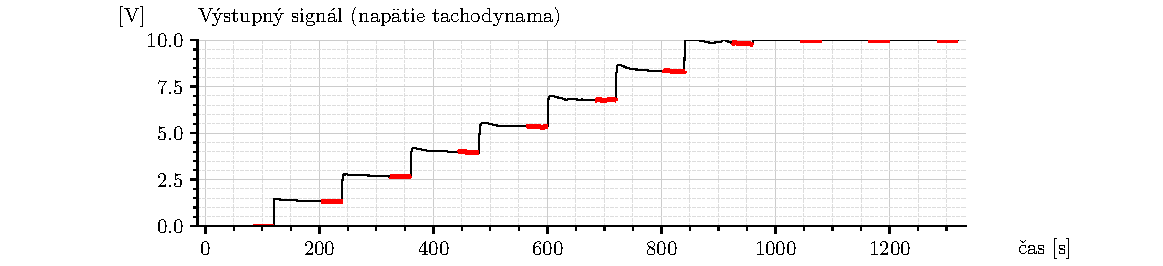
\includegraphics{fj_02_data_pot0_panel_1.pdf}
        }

        \makebox[\textwidth][c]{%
        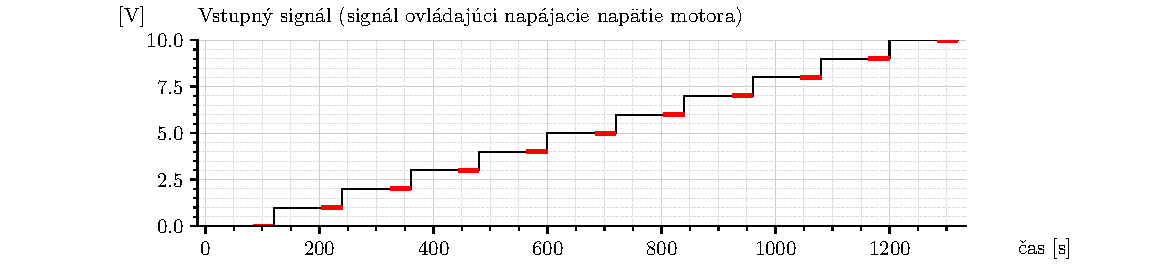
\includegraphics{fj_02_data_pot0_panel_3.pdf}
        }

        % \figcaption{ 
        \caption{
            % 
        }
        \label{fj_02_data_pot0}
    }%vbox

\end{figure}
% \end{center}







\subsection{Nameraná prevodová charakteristika}

Vyňaté úseky je možné zlúčiť do jedného dátového súboru. Obsahuje len hodnoty vstupného signálu a výstupného signálu, pre ktoré je možné konštatovať, že zodpovedajú ustálenému stavu. Takéto dáta charakterizujú systém v ustálených stavoch.

Grafické znázornenie uvedených dát tak, že na x-ovej osi sú hodnoty vstupného signálu v ustálenom stave a na y-ovej osi sú prislúchajúce hodnoty výstupného signálu v~ustálenom stave, je vlastne grafickým vyjadrením nameranej prevodovej charakteristiky. Nameraná prevodová charakteristika je znázornená na obrázku \ref{fj_03_data_pot0_panel_1}.

Pre lepšiu ilustráciu, že uvedený dataset neobsahuje takpovediac len niekoľko bodov, ale že každý ustálený stav je reprezentovaný viacerými hodnotami, je na obrázku \ref{fj_03_data_pot0_panel_2} zobrazený detail pre zvolenú hodnotu vstupného signálu.

% \begin{center}
    \begin{figure}[t]

    \vbox{%
        \makebox[\textwidth][c]{%
        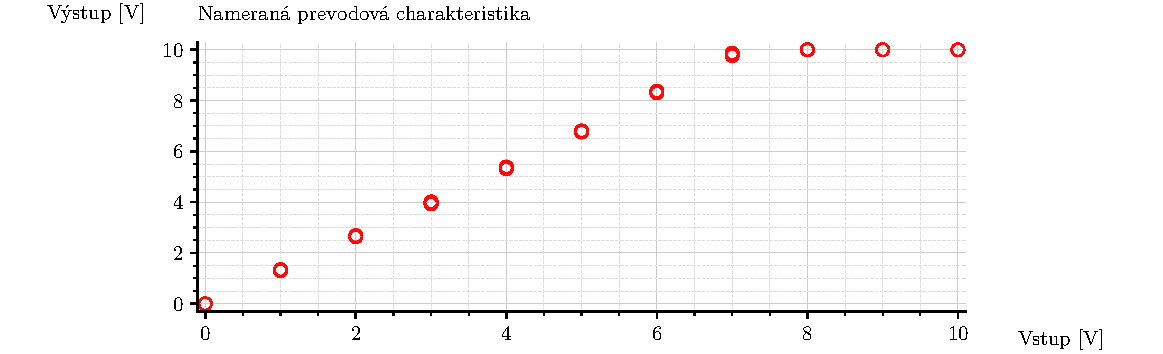
\includegraphics{fj_03_data_pot0_panel_1.pdf}
        }

        % \figcaption{ 
        \caption{
            Nameraná prevodová charakteristika pre prevádzkovú podmienku $0$ [V]. 
        }
        \label{fj_03_data_pot0_panel_1}
    }%vbox

\end{figure}
% \end{center}


% \begin{center}
    \begin{figure}[t]

    \vbox{%
        \makebox[\textwidth][c]{%
        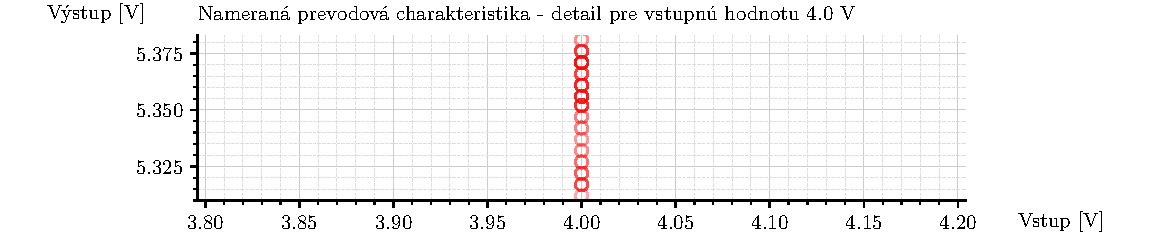
\includegraphics{fj_03_data_pot0_panel_2.pdf}
        }

        % \figcaption{ 
        \caption{
            % 
        }
        \label{fj_03_data_pot0_panel_2}
    }%vbox

\end{figure}
% \end{center}











% \newpage
\clearpage
% \pagebreak

\section{Príloha - vizualizácia získaných dát}


\vspace{-6pt}

\paragraph{Meranie ustálených hodnôt pri prevádzkovej podmienke 0 [V]}

Pozri obrázok \ref{fj_01_data_pot0}.

\vspace{-6pt}


\paragraph{Meranie ustálených hodnôt pri prevádzkovej podmienke 1 [V]}

\begin{center}

    \vbox{%
        \makebox[\textwidth][c]{%
        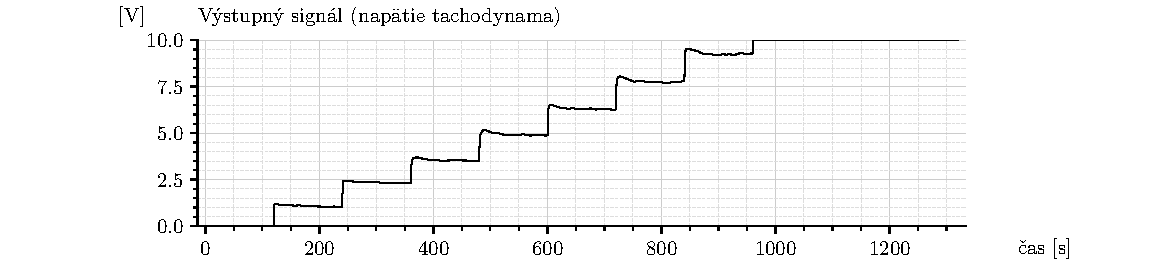
\includegraphics{fj_01_data_pot1_panel_1.pdf}
        }

        \makebox[\textwidth][c]{%
        
\includegraphics{fj_01_data_pot1_panel_3.pdf}
        }

        \makebox[\textwidth][c]{%
        
\includegraphics{fj_01_data_pot1_panel_2.pdf}
        }

        \figcaption{ 
            Získané dáta pre vstupný signál a výstupný signál systému LMOT pri manuálne nastavenej prevádzkovej podmienke $1$ [V].
        }
        \label{fj_01_data_pot1}
    }%vbox

\end{center}

% \vfill

\vspace{-6pt}

\paragraph{Meranie ustálených hodnôt pri prevádkovej podmienke 2 [V]}

\begin{center}

    \vbox{%
        \makebox[\textwidth][c]{%
        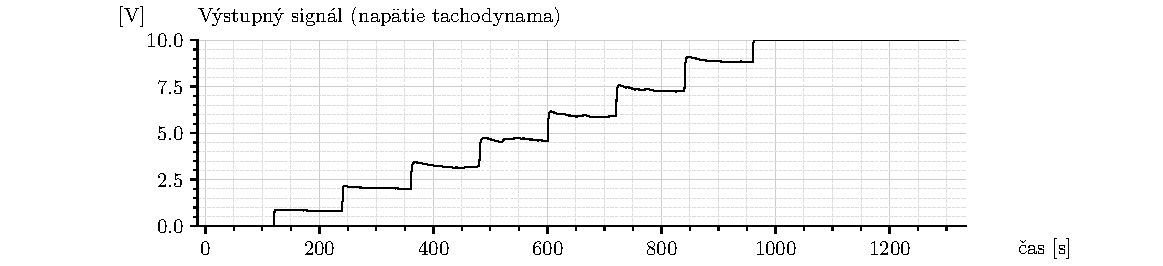
\includegraphics{fj_01_data_pot2_panel_1.pdf}
        }

        \makebox[\textwidth][c]{%
        
\includegraphics{fj_01_data_pot2_panel_3.pdf}
        }

        \makebox[\textwidth][c]{%
        
\includegraphics{fj_01_data_pot2_panel_2.pdf}
        }

        \figcaption{ 
            Získané dáta pre vstupný signál a výstupný signál systému LMOT pri manuálne nastavenej prevádzkovej podmienke $2$ [V].
        }
        \label{fj_01_data_pot2}
    }%vbox

\end{center}

% \vfill

% \phantom{}

\pagebreak



\paragraph{Meranie ustálených hodnôt pri prevádzkovej podmienke 3 [V]}

\begin{center}

    \vbox{%
        \makebox[\textwidth][c]{%
        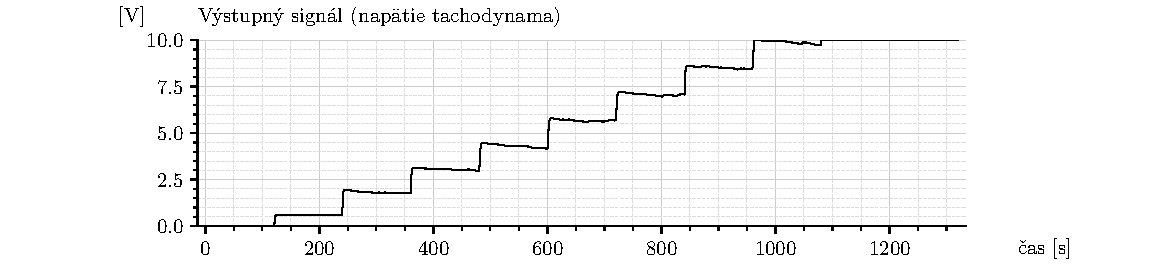
\includegraphics{fj_01_data_pot3_panel_1.pdf}
        }

        \makebox[\textwidth][c]{%
        
\includegraphics{fj_01_data_pot3_panel_3.pdf}
        }

        \makebox[\textwidth][c]{%
        
\includegraphics{fj_01_data_pot3_panel_2.pdf}
        }

        \figcaption{ 
            Získané dáta pre vstupný signál a výstupný signál systému LMOT pri manuálne nastavenej prevádzkovej podmienke $3$ [V].
        }
        \label{fj_01_data_pot3}
    }%vbox

\end{center}

\vfill

\paragraph{Meranie ustálených hodnôt pri prevádzkovej podmienke 4 [V]}

\begin{center}

    \vbox{%
        \makebox[\textwidth][c]{%
        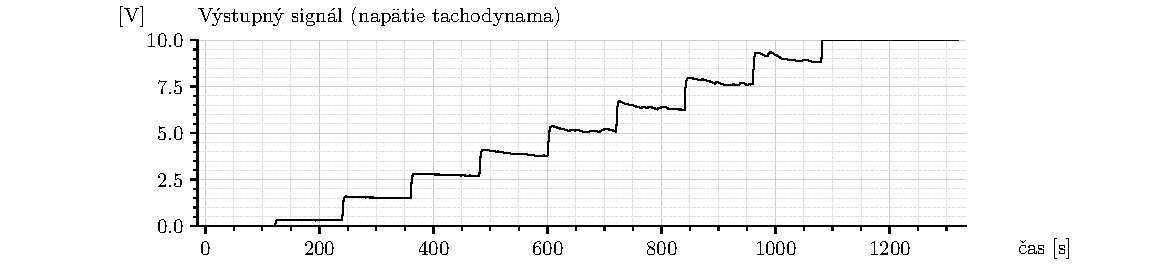
\includegraphics{fj_01_data_pot4_panel_1.pdf}
        }

        \makebox[\textwidth][c]{%
        
\includegraphics{fj_01_data_pot4_panel_3.pdf}
        }

        \makebox[\textwidth][c]{%
        
\includegraphics{fj_01_data_pot4_panel_2.pdf}
        }

        \figcaption{ 
            Získané dáta pre vstupný signál a výstupný signál systému LMOT pri manuálne nastavenej prevádzkovej podmienke $4$ [V].
        }

        \label{fj_01_data_pot4}
    }%vbox

\end{center}

\vfill

\phantom{}

\pagebreak

\paragraph{Meranie ustálených hodnôt pri prevádzkovej podmienke 5 [V]}

\begin{center}

    \vbox{%
        \makebox[\textwidth][c]{%
        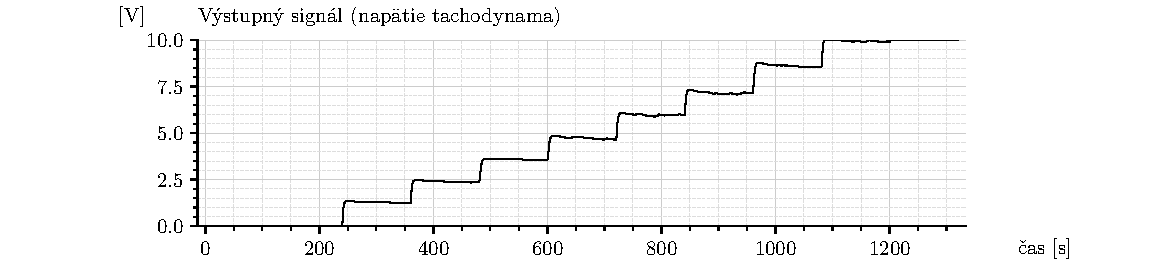
\includegraphics{fj_01_data_pot5_panel_1.pdf}
        }

        \makebox[\textwidth][c]{%
        
\includegraphics{fj_01_data_pot5_panel_3.pdf}
        }

        \makebox[\textwidth][c]{%
        
\includegraphics{fj_01_data_pot5_panel_2.pdf}
        }

        \figcaption{ 
            Získané dáta pre vstupný signál a výstupný signál systému LMOT pri manuálne nastavenej prevádzkovej podmienke $5$ [V].
        }

        \label{fj_01_data_pot5}

    }%vbox

\end{center}

\vfill

\paragraph{Meranie ustálených hodnôt pri prevádzkovej podmienke 6 [V]}

\begin{center}

    \vbox{%
        \makebox[\textwidth][c]{%
        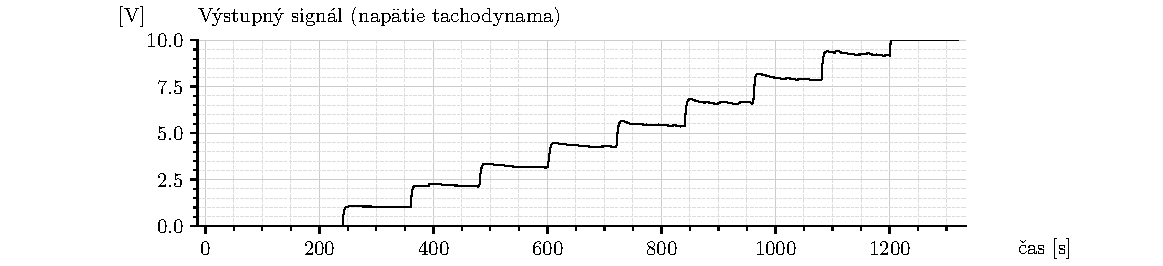
\includegraphics{fj_01_data_pot6_panel_1.pdf}
        }

        \makebox[\textwidth][c]{%
        
\includegraphics{fj_01_data_pot6_panel_3.pdf}
        }

        \makebox[\textwidth][c]{%
        
\includegraphics{fj_01_data_pot6_panel_2.pdf}
        }

        \figcaption{ 
            Získané dáta pre vstupný signál a výstupný signál systému LMOT pri manuálne nastavenej prevádzkovej podmienke $6$ [V].
        }

        \label{fj_01_data_pot6}

    }%vbox

\end{center}

\vfill

\phantom{}

\pagebreak

\paragraph{Meranie ustálených hodnôt pri prevádzkovej podmienke 7 [V]}

\begin{center}

    \vbox{%
        \makebox[\textwidth][c]{%
        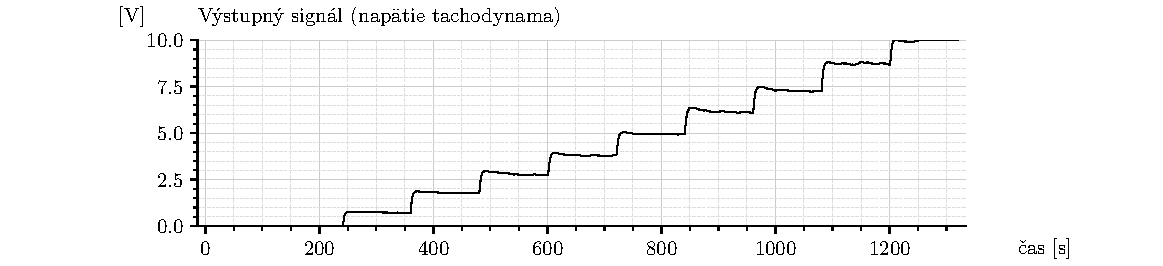
\includegraphics{fj_01_data_pot7_panel_1.pdf}
        }

        \makebox[\textwidth][c]{%
        
\includegraphics{fj_01_data_pot7_panel_3.pdf}
        }

        \makebox[\textwidth][c]{%
        
\includegraphics{fj_01_data_pot7_panel_2.pdf}
        }

        \figcaption{ 
            Získané dáta pre vstupný signál a výstupný signál systému LMOT pri manuálne nastavenej prevádzkovej podmienke $7$ [V].
        }

        \label{fj_01_data_pot7}

    }%vbox

\end{center}

\vfill

\paragraph{Meranie ustálených hodnôt pri prevádzkovej podmienke 8 [V]}

\begin{center}

    \vbox{%
        \makebox[\textwidth][c]{%
        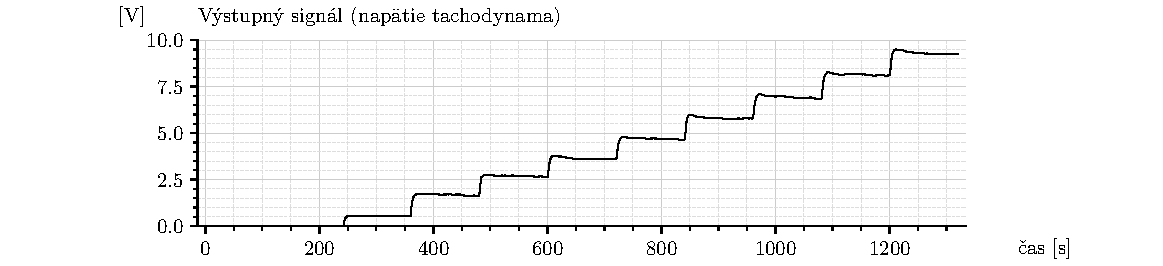
\includegraphics{fj_01_data_pot8_panel_1.pdf}
        }

        \makebox[\textwidth][c]{%
        
\includegraphics{fj_01_data_pot8_panel_3.pdf}
        }

        \makebox[\textwidth][c]{%
        
\includegraphics{fj_01_data_pot8_panel_2.pdf}
        }

        \figcaption{ 
            Získané dáta pre vstupný signál a výstupný signál systému LMOT pri manuálne nastavenej prevádzkovej podmienke $8$ [V].
        }

        \label{fj_01_data_pot8}

    }%vbox

\end{center}

\vfill

\phantom{}

\pagebreak

\paragraph{Meranie ustálených hodnôt pri prevádzkovej podmienke 9 [V]}

\begin{center}

    \vbox{%
        \makebox[\textwidth][c]{%
        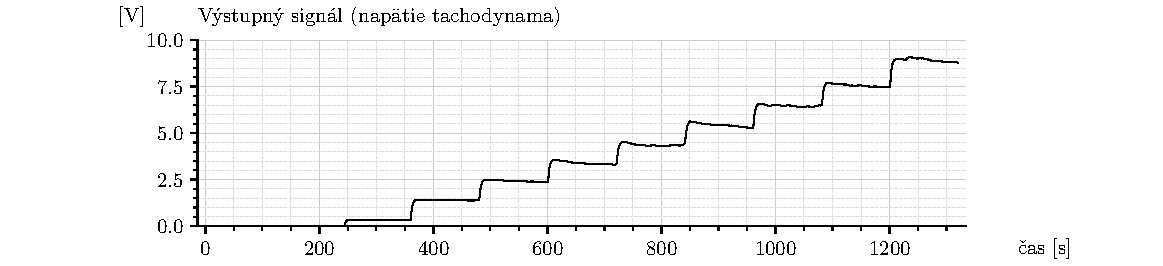
\includegraphics{fj_01_data_pot9_panel_1.pdf}
        }

        \makebox[\textwidth][c]{%
        
\includegraphics{fj_01_data_pot9_panel_3.pdf}
        }

        \makebox[\textwidth][c]{%
        
\includegraphics{fj_01_data_pot9_panel_2.pdf}
        }

        \figcaption{ 
            Získané dáta pre vstupný signál a výstupný signál systému LMOT pri manuálne nastavenej prevádzkovej podmienke $9$ [V].
        }

        \label{fj_01_data_pot9}

    }%vbox

\end{center}

\vfill

\paragraph{Meranie ustálených hodnôt pri prevádzkovej podmienke 10 [V]}

\begin{center}

    \vbox{%
        \makebox[\textwidth][c]{%
        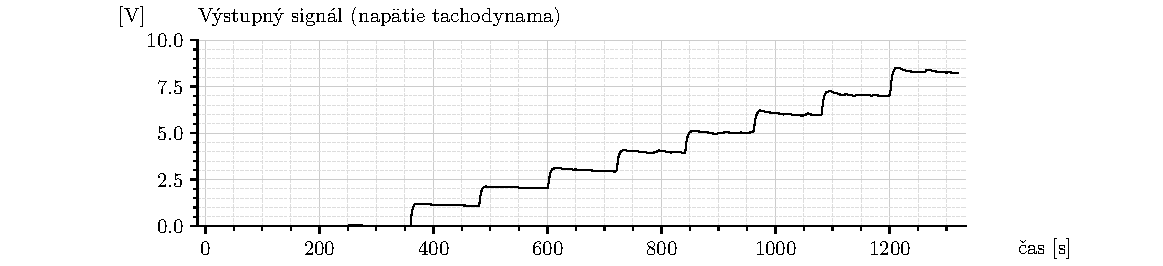
\includegraphics{fj_01_data_pot10_panel_1.pdf}
        }

        \makebox[\textwidth][c]{%
        
\includegraphics{fj_01_data_pot10_panel_3.pdf}
        }

        \makebox[\textwidth][c]{%
        
\includegraphics{fj_01_data_pot10_panel_2.pdf}
        }

        \figcaption{ 
            Získané dáta pre vstupný signál a výstupný signál systému LMOT pri manuálne nastavenej prevádzkovej podmienke $10$ [V].
        }

        \label{fj_01_data_pot10}

    }%vbox

\end{center}

\vfill

\phantom{}
















\clearpage


\dirtree{%
 .1 .
 .2 ML.
 .3 dataRepo.
 .4 dataSet01.
 .5 \dots.
 .4 rawData.
 .5 \dots.
 .3 SteadyStateChar.slx.
 .3 logsout\_basicPlot.m.
 .3 measurementSetup.m.
 .2 PY.
 .3 dataRepo.
 .4 \dots.
 .3 datajobs.
 .4 dataJob\_02.py.
 .3 fig.
 .4 \dots.
 .3 figjobs.
 .4 figFcns\_TeX.py.
 .4 figJob\_01.py.
 .4 figJob\_02.py.
 .4 figJob\_03.py.
 .3 dataJob\_SSChar.ipynb.
 .2 TeX.
 .3 COMMONFILES.
 .4 \dots.
 .3 KUTdev250624.pdf.
 .3 KUTdev250624.tex.
}



% -----------------------------------------------------------------------------

\end{document}

% -----------------------------------------------------------------------------